\NeedsTeXFormat{LaTeX2e}

\documentclass[prb,twocolumn,showpacs,superscriptaddress]{revtex4}

\usepackage{epsfig}
\usepackage{amsmath,amssymb}
\usepackage{graphicx}
\usepackage{footnote}
\usepackage{grffile}
\usepackage{color}
\usepackage{dsfont}
\usepackage{mathtools}
\usepackage{verbatim}
%\usepackage{todonotes}
%\usepackage{booktabs}
%\usepackage[caption=false]{subfig}
%\usepackage[all]{xy}


% --- Useful commands

\newcommand{\todo}[1]{\textcolor{red}{\textbf{[TODO: #1]}}}
%\newcommand{\grtodo}[1]{\todo[inline,backgroundcolor=blue!20!white]{\textcolor{black}{{\bf GR}: #1}}}

\newcommand{\tw}{\textwidth}
\newcommand{\cw}{\columnwidth}

\newcommand{\mc}[1]{\mathcal{#1}}

\newcommand{\RE}{\operatorname{Re}}
\newcommand{\IM}{\operatorname{Im}}

\newcommand{\ceq}[1]{Eq.~(\ref{eq:#1})}
\newcommand{\cfg}[1]{Fig.~\ref{fig:#1}}

\newcommand{\nn}{\nonumber}
\newcommand{\pdag}{{\phantom{\dagger}}}

\newcommand{\vp}{\varphi}
\newcommand{\vpb}{\bar{\varphi}}

\newcommand{\ud}{{ \uparrow\downarrow }}		% Up-Down
\newcommand{\udc}{{ \overline{\uparrow\downarrow} }}	% Up-Down-Cross
\newcommand{\uu}{{ \uparrow\uparrow }}			% Up-Up

\newcommand{\xph}{{ \overline{ph} }}			% Exchange Particle-hole

\newcommand{\K}{\mc{K}_1}				% K 1
\newcommand{\KUD}{\mc{K}_{1,\ud}}			% K 1 ud
\newcommand{\KPP}{\mc{K}_{1, pp}}			% K 1 pp
\newcommand{\KPH}{\mc{K}_{1, ph}}			% K 1 ph
\newcommand{\KXPH}{\mc{K}_{1, \xph}}			% K 1 xph
\newcommand{\KPPUD}{\mc{K}_{1, pp, \ud}}		% K 1 pp ud
\newcommand{\KPHUD}{\mc{K}_{1, ph, \ud}}		% K 1 ph ud
\newcommand{\KXPHUD}{\mc{K}_{1, \xph, \ud}}		% K 1 xph ud
\newcommand{\KK}{\mc{K}_2}				% K 2
\newcommand{\KKUD}{\mc{K}_{2,\ud}}			% K 2 ud
\newcommand{\KKB}{\overline{\mc{K}}_2}			% K 2 bar
\newcommand{\KKPP}{\mc{K}_{2, pp}}			% K 2 pp
\newcommand{\KKBPP}{\overline{\mc{K}}_{2, pp}}		% K 2 bar pp
\newcommand{\KKPH}{\mc{K}_{2, ph}}			% K 2 ph
\newcommand{\KKBPH}{\overline{\mc{K}}_{2, ph}}		% K 2 bar ph
\newcommand{\KKXPH}{\mc{K}_{2, \xph}}			% K 2 xph
\newcommand{\KKBXPH}{\overline{\mc{K}}_{2, \xph}}	% K 2 bar xph
\newcommand{\KKPPUD}{\mc{K}_{2, pp, \ud}}		% K 2 pp ud
\newcommand{\KKPHUD}{\mc{K}_{2, ph, \ud}}		% K 2 ph ud
\newcommand{\KKXPHUD}{\mc{K}_{2, \xph, \ud}}		% K 2 xph ud
\newcommand{\R}{\mc{R}} 				% Rest-function
\newcommand{\RUD}{\mc{R}_{\ud}}				% Rest-function ud
\newcommand{\RPP}{\mc{R}_{pp}} 				% Rest-function pp
\newcommand{\RPH}{\mc{R}_{ph}} 				% Rest-function ph
\newcommand{\RXPH}{\mc{R}_{\xph}} 			% Rest-function ph

\DeclareMathOperator*{\sumint}{%
   \mathchoice%
  {\ooalign{$\displaystyle\sum$\cr\hidewidth$\displaystyle\int$\hidewidth\cr}}
  {\ooalign{\raisebox{.14\height}{\scalebox{.7}{$\textstyle\sum$}}\cr\hidewidth$\textstyle\int$\hidewidth\cr}}
  {\ooalign{\raisebox{.2\height}{\scalebox{.6}{$\scriptstyle\sum$}}\cr$\scriptstyle\int$\cr}}
  {\ooalign{\raisebox{.2\height}{\scalebox{.6}{$\scriptstyle\sum$}}\cr$\scriptstyle\int$\cr}}
}


\begin{document}

\title{Status report about charge instability}


\newcommand{\MPIStutt}{\affiliation{Max-Planck-Institute for Solid State Research, 70569 Stuttgart, Germany}}

\author{Demetrio Vilardi }   \MPIStutt 

\author{Ciro Taranto} 		 \MPIStutt

\author{Walter Metzner }     \MPIStutt 



\begin{abstract}

We collect some results obtained by means of different implementations of fRG equations using a full frequency dependent vertex. 
It emerges a very peaked structure in the charge-channel for finite frequency-transfer, that in some region of the parameter space becomes divergent. Such a divergence has no obvious physical interpretation.  
The peaked structure seems to be characteristic of the frequency dependence of the vertex, as it is shown by means of simpled diagrams. 
On the other hand the \emph{divergence} of this structure may be very sensitive to the detailed structure of the Green's function used in the calculation, i.e., very sensitive to the use, or not, of dressed propagators, even when the correction to the self-energy appear to be small (i.e., self-energy Fermi liquid-like).  

\end{abstract}

\maketitle

\section{fRG without self-energy} 				
\label{sec:frgnoself}
  The results shown in this section are obtained in standard fRG using an interaction cutoff: $G_0^\Lambda = \Lambda G_0$. The calculations are performed on the Matsubara frequency axis for temperature $T=0,08 t$, where $t$ is the nearest neighbors hopping.  

Besides the vertex, we have computed the susceptibilities, whose divergences follow the vertex ones. 

\subparagraph{Technicalities}
\begin{itemize} 

\item The vertex was decomposed in channels (magnetic, density, and superconducting) as usual in the literature. 

\item We have previously shown that the full frequency dependence of the vertex can change drastically the resutls (as opposed for example to a bosonic frequency transfer decomposition), and hence we kept all the frequencies in a finite box. 

\item The momentum dependence of the vertex is treated by means of a form factor decomposition, while keeping 29 patches in the respective bosonic momentum transfer . The critical scale is fixed by the condition that the absolute value of one of the channels exceeds a value of 300$D$, $D=4t$. 


\item In all the calculations in this section we did not include any self-energy feedback. The calculation of the self-energy, with a full frequency dependence vertex  is ongoing work, and needs more testing. Some results are presented in the following paragraphs. 
 
If not otherwise specified we measure energies in units of $D=4t$, i.e., $t'=0.1$ corresponds to $t'=0.4t$.
\end{itemize} 
 
\subparagraph{Results} 

In Fig \ref{phasediag_van_hove} and \ref{phasediag_van_hove_plus} we show  a putative phase diagram, for, respectively, van Hove filling, and van Hove filling plus 7\%. 

The fininte temperature acts as a cutoff for divergencies in the bare bubble. 

\begin{figure}
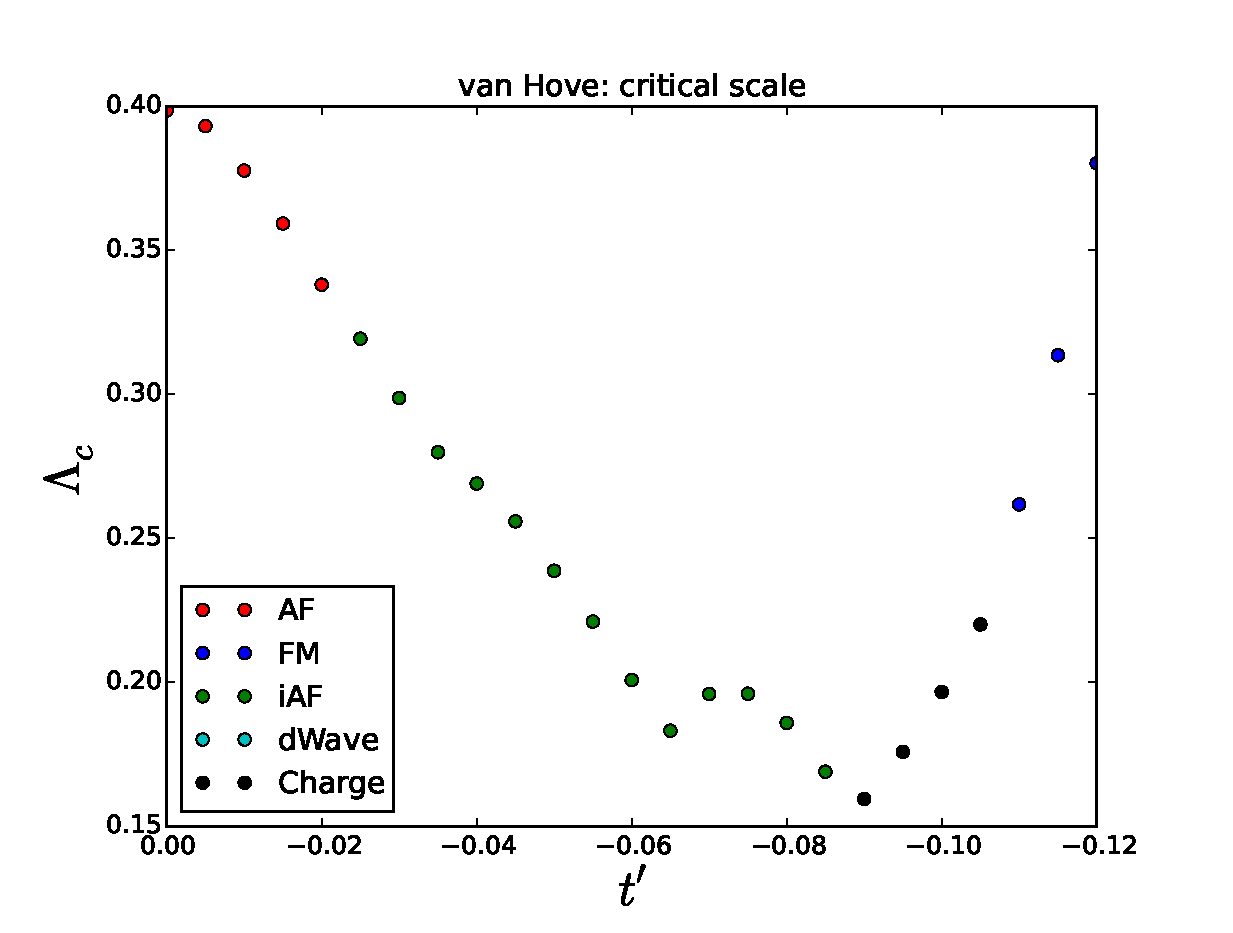
\includegraphics[scale=0.8]{vanHove_scan_critical_lambda_phi.eps}
\caption{Critical scale in full frequency fRG (interaction cutoff) as a function of the nearest neighbors hopping and for van Hove filling. The color of the symbol indicates the kind of instability that is realized.  } \label{phasediag_van_hove}

\end{figure}

\begin{figure}
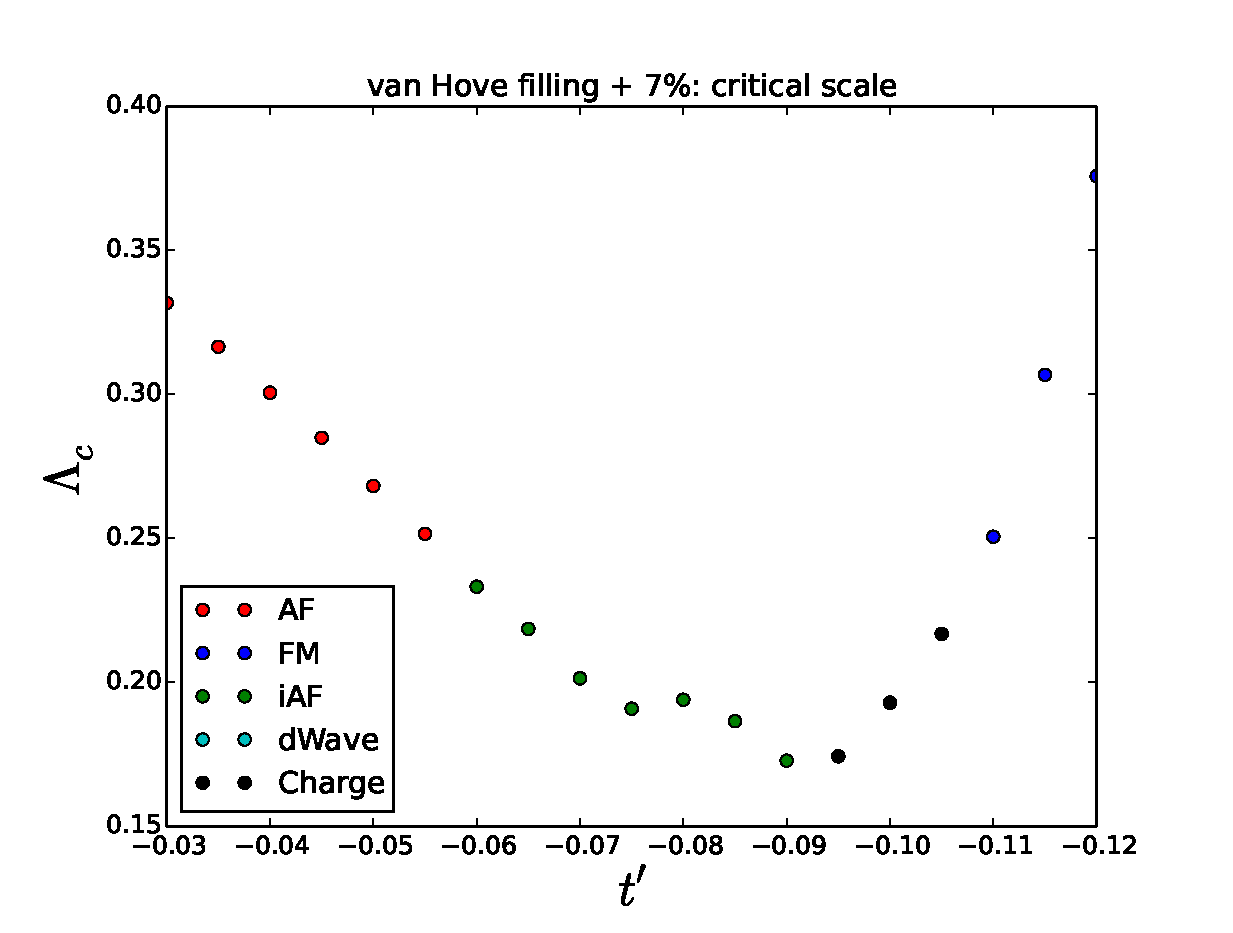
\includegraphics[scale=0.8]{vanHove_plus_scan_critical_lambda_phi.eps}
\caption{Critical scale in full frequency fRG (interaction cutoff) as a function of the nearest neighbors hopping and for van Hove filling + 7 \% . The color of the symbol indicates the kind of instability that is realized.} 
\label{phasediag_van_hove_plus} 
\end{figure}

In the spirit of the "interaction cutoff" the critical scale can be associated with the maximal value of the interaction $U_{\mathrm{flow}}\approx(1-\Lambda)^2 U$ \textbf{check if there is the square} for which the flow would converge. 
In a purely weak coupling scenario one can assume a monothonic relation between the interaction value and the critical temperature, and hence we can qualitatively associate the critical scale whith a critical temperature. In this sense our results are consistent with those reported in the literature. 

We hava double-checked the consistency of our results by also considering a frequency selective cuffoff, which substitutes: $i\omega \rightarrow i\mathrm{sign} \omega \sqrt{\omega^2+\Lambda^2}$. 

\begin{figure}
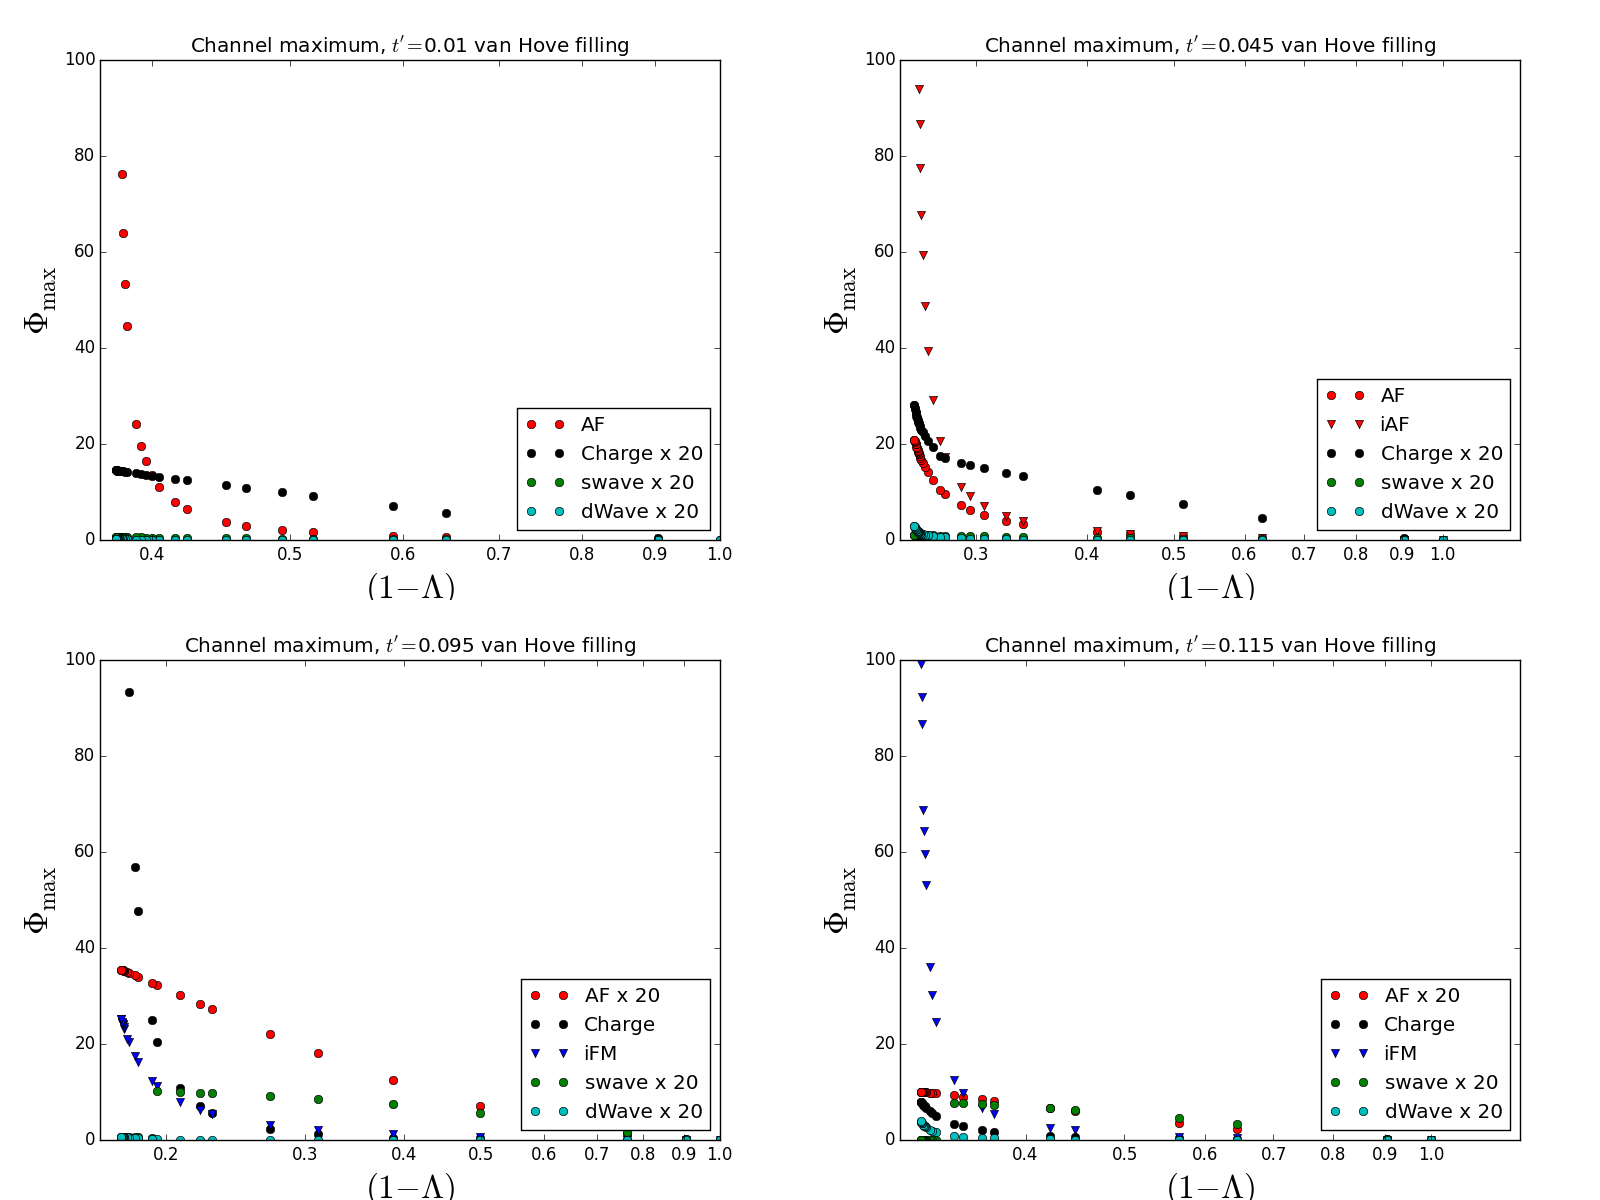
\includegraphics[scale=0.25]{images/vanhovelam.png}
\caption{Flow of the maximum of the absolute value of each channel for differnt values of $t'$ and at van Hove filling.
} 
\label{lamvan} 
\end{figure}

\begin{figure}
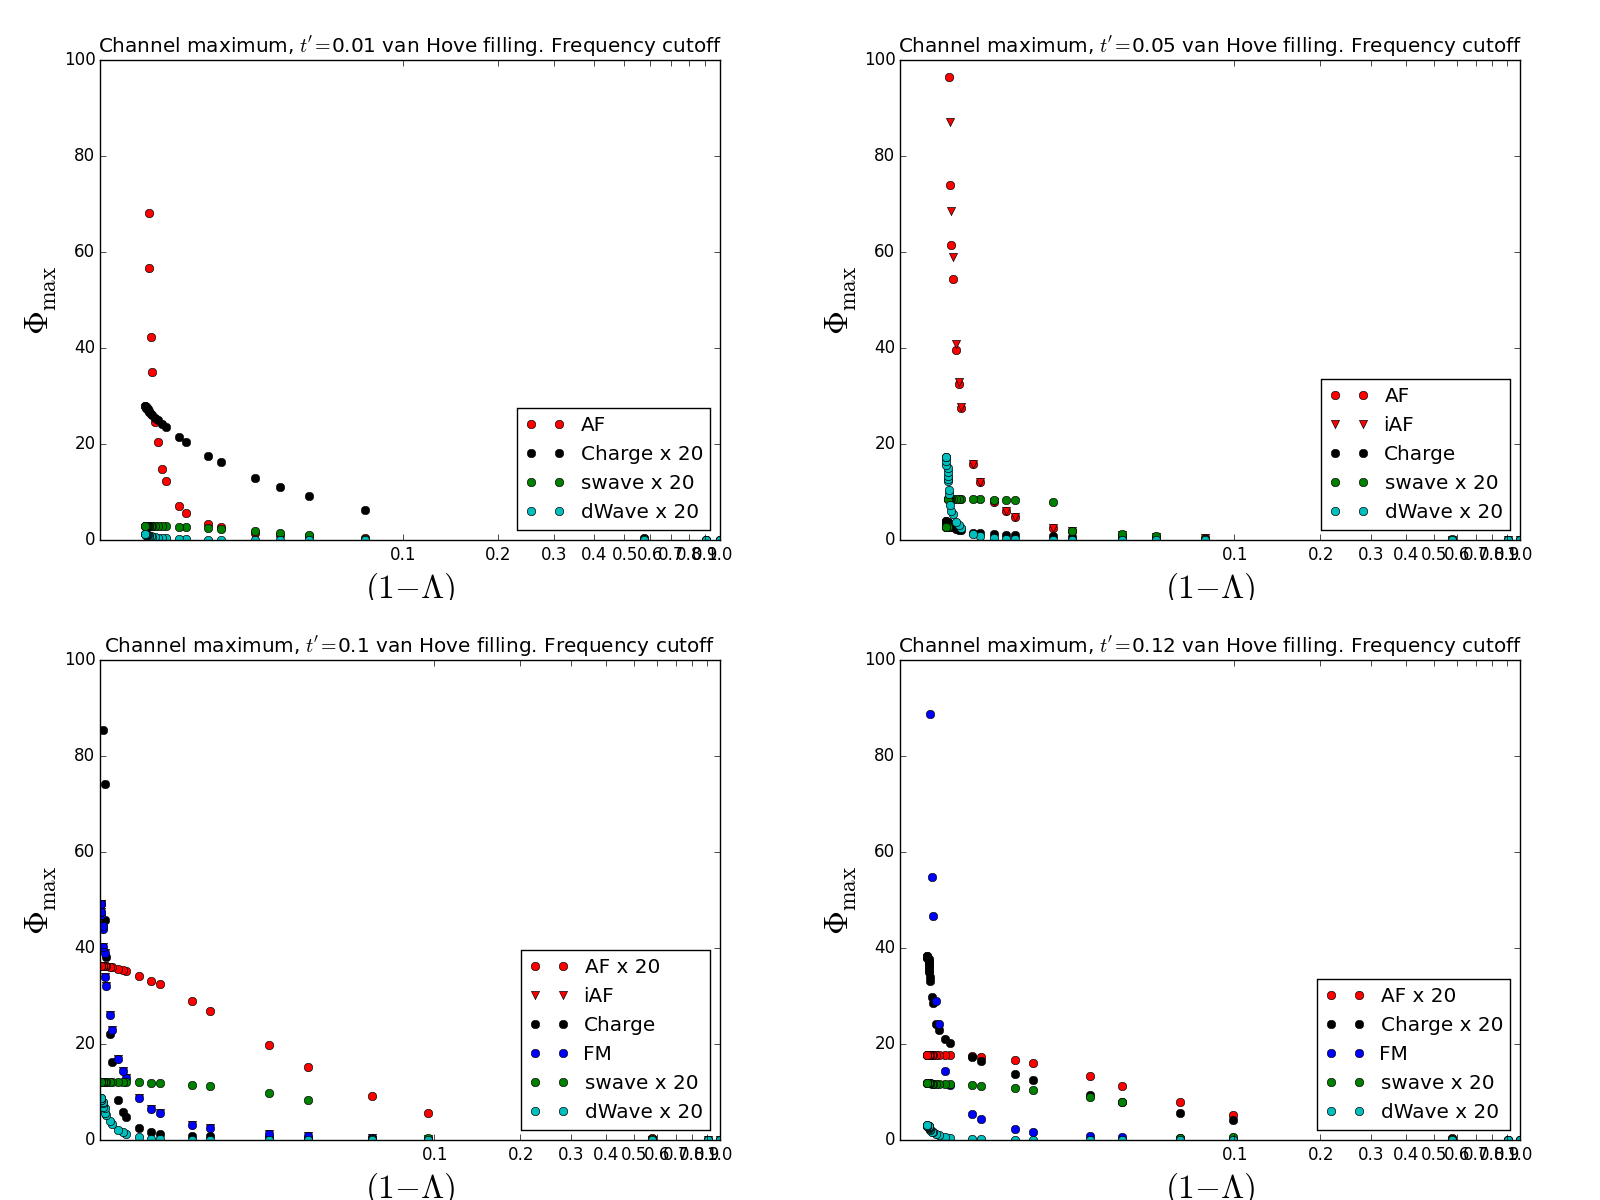
\includegraphics[scale=0.25]{images/freqvanhove.png}
\caption{Flow of the maximum of the absolute value of each channel for differnt values of $t'$ and at van Hove filling. } 
\label{freqlam} 
\end{figure}

\begin{figure}
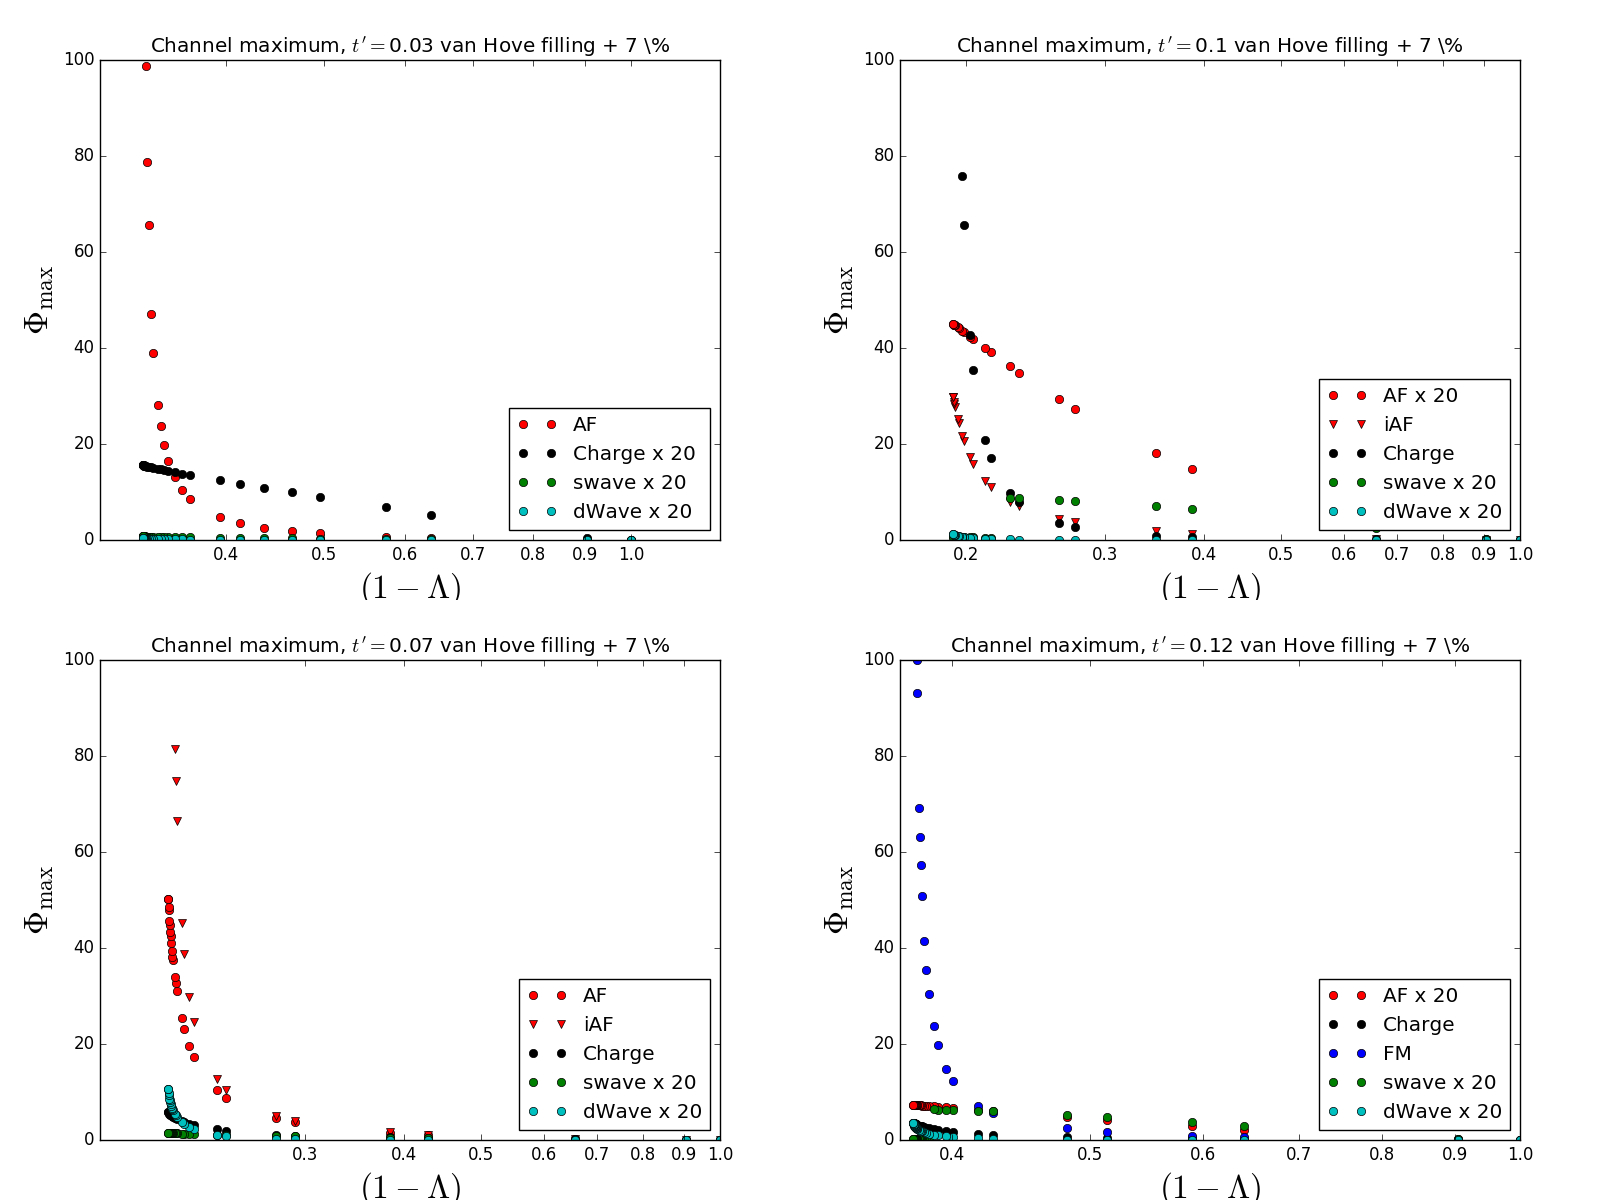
\includegraphics[scale=0.25]{images/vanhovepluslambda.png}
\caption{Flow of the maximum of the absolute value of each channel for differnt values of $t'$ and at van Hove filling $+7 \%$.
} 
\label{lamvanplus} 
\end{figure}

\subparagraph{Charge instability problem}

We call \textit{charge instability problem} the divergence of the charge component of the vertex for a finite bosonic frequency transfer, i.e. $\Omega_{ph} = 2\pi/\beta$, as already reported in the literature by Husemann \emph{et al}. 
\begin{itemize}
\item The charge channel diverges for a region of filling/next neighbors hopping between iAF and FM. In static fRG in this region one can find $d$wave superconductivity, usually at much lower scales. 
\item The \textit{divergence} of the channel is associated with a very specific \textit{frequency-structure}. The frequency-structure can be explained (section about perpendicular ladders), it's divergence instead is unphysical. 
\item The charge-channel divergence arises also in DMF$^2$RG, where the DMFT self-energy is already included in the flow equations. 
\item Introducing a \emph{full} self-energy feedback the in DMF$^2$RG the problem seems to be suppressed. 
\item Similar observations in fRG, with major approximations on the self energy feedback.
\item The divergence is very localized in frequency space. Nevertheless it is sufficient to induce large values of the charge susceptibility, with a maximum at finite frequency transfer.    
\end{itemize} 
 
\textbf{Here include some color plots of the charge channel vs magnetic channel}



%\section{DMF$^2$RG without self-energy}	
%\label{sec:dmf2rgnoself}
  %In this section we present results obtained with DMF$^2$RG.  We use an interpolative cutoff: $[G_0^\Lambda(\mathbf{k},\omega)]^{-1} = (1-\Lambda)[G_0(\mathbf{k},\omega)]^{-1}+\Lambda \mathcal{G}_{\mathrm{AIM}}(\omega)$, ($\mathcal{G}_{\mathrm{AIM}}$ is the propagator of the DMFT self-consistent Anderson impurity model associated with the lattice under consideration. The initial condition for the vertex and the self-energy is per se frequency dependent. 
Apart for this, the implementation is equivalent to the one used in fRG, i.e., same frequency and momentum treatments. 
The self-energy is however better-behaved, compared to the fRG situation: we speculate that this is a consequence of the fact that the flow only has to compute the deviation from the DMFT self-energy. Hence the results with the self energy feedback of this section are numerically more stable.  

The results presented here are (in the usual fRG units) for $U=6.8t$, $T=0.08t$, filling $n=0.85$, and next neighbors hopping $t'=-0.3$.  
\begin{figure}
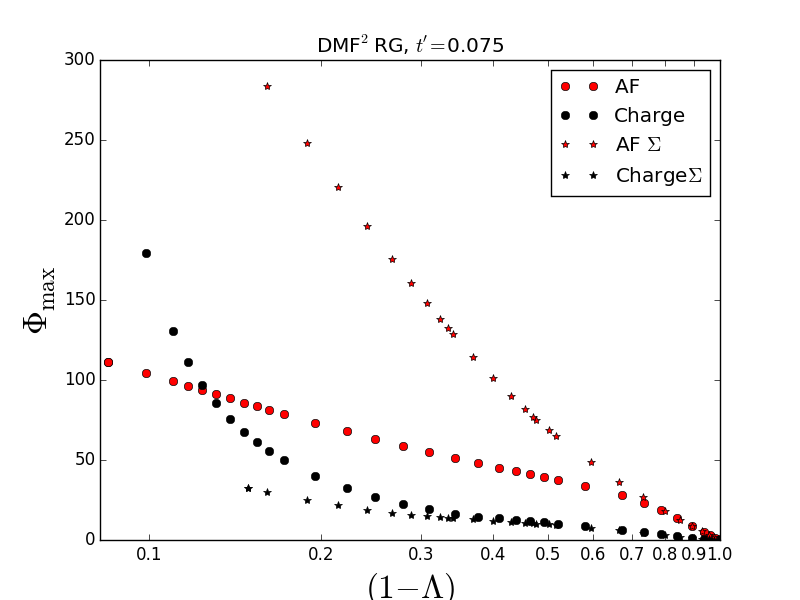
\includegraphics[scale=0.70]{images/dmf2rglam.png}
\caption{Flow of the maximum absolute value of the real part of the magnetic and charge channel in DMF$^2$RG, with and without self-energy feedback.} \label{dmf2rglam}
\end{figure}

\begin{figure}
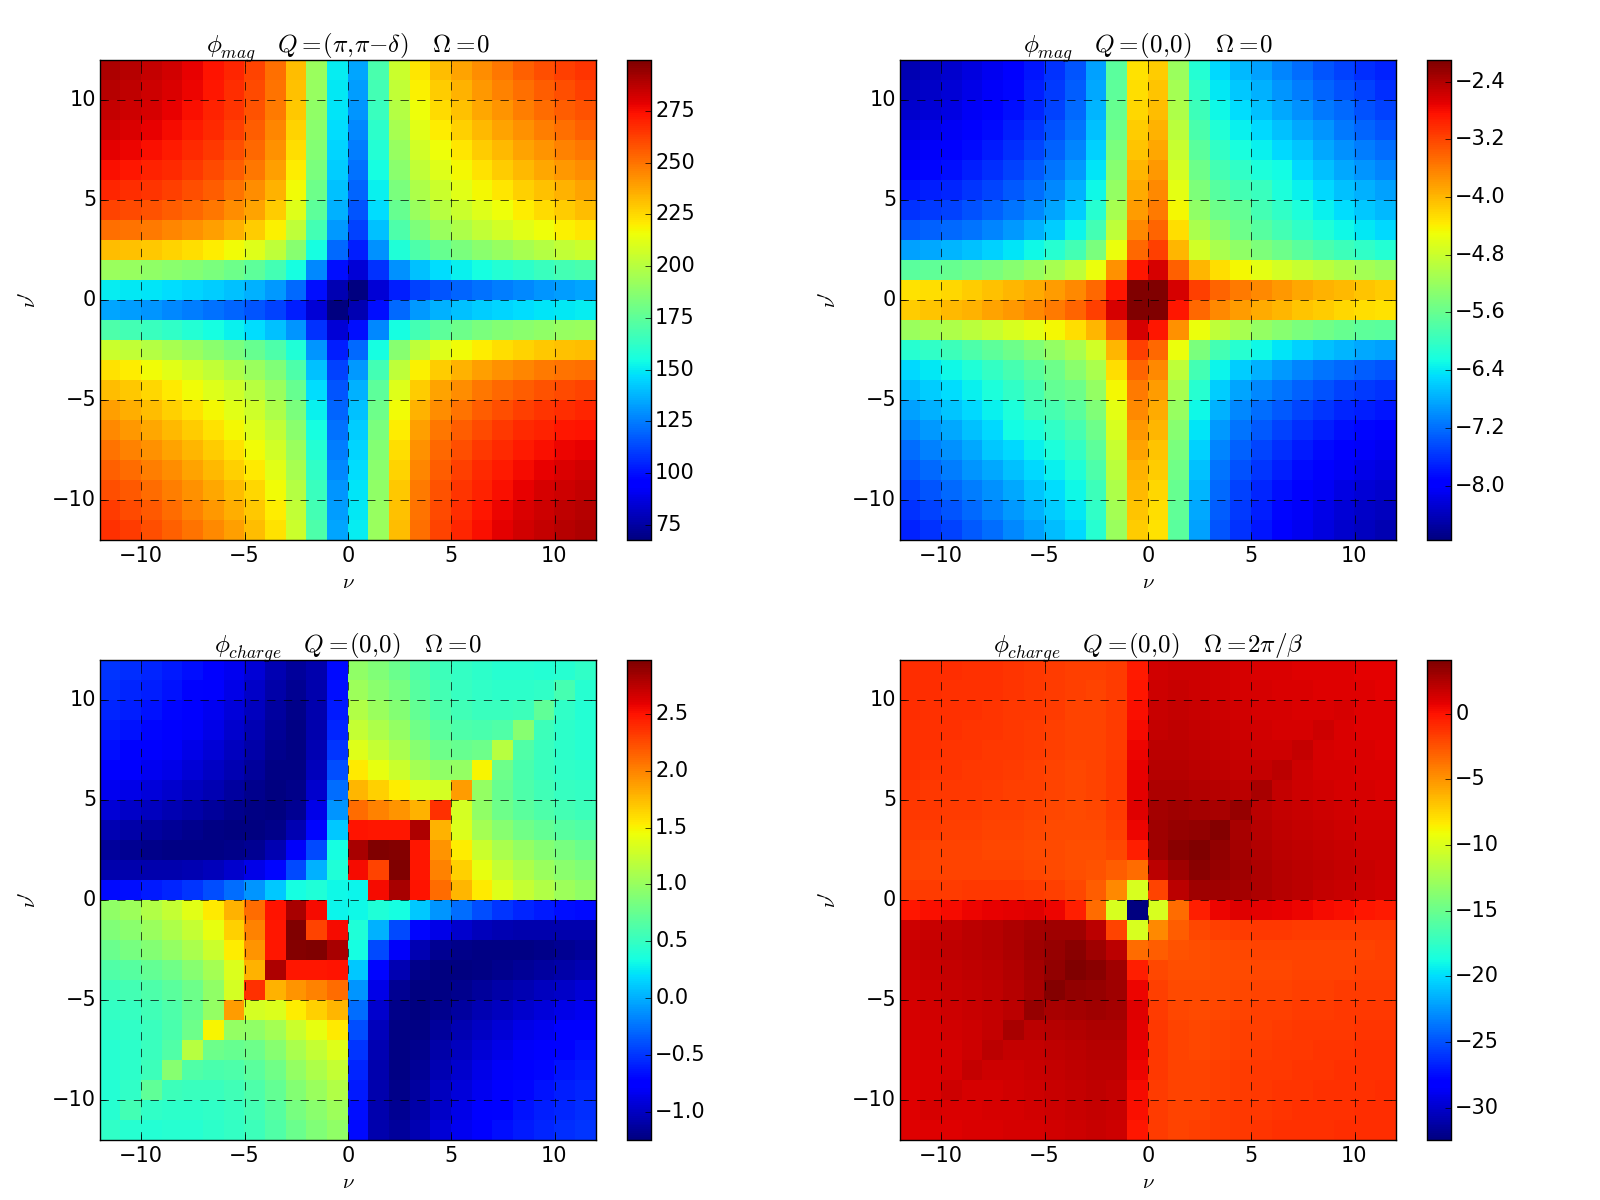
\includegraphics[scale=0.25]{images/Merged_dmf2rg_se.png}
\caption{Frequency dependence of the $\Phi$'s in DMF$^2$RG with self-energy feedback.} \label{dmf2rfreq}
\end{figure}

\subparagraph{Results} 
\begin{itemize}

\item The charge channel instability is present also in DMF$^2$RG, even if the DMFT self energy broadens the Fermi surface, see Fig. \ref{dmf2rflam}.  

\item At large coupling, and without self-energy feedback, we have observed a divergence of the charge channel for any parameter set studied (excluding the case of particle-hole symmetry)$\rightarrow$ up to now the charge-channel divergence is the bottleneck of DMF$^2$RG;  

\item While in fRG the charge divergence seemed to be associated to a crossover from iAF to FM, the charge channel divergence arises in a  AF dominated region;
 
\item The richer frequency structure of the magnetic channel (as compared to the one of fRG) can be understood in terms of ladder diagrams: the same frequency structure arises from Bethe-Salpeter-like equations using the DMFT irreducible vertex, see Fig. \ref{dmf2rfreq}

\end{itemize}

\begin{figure}
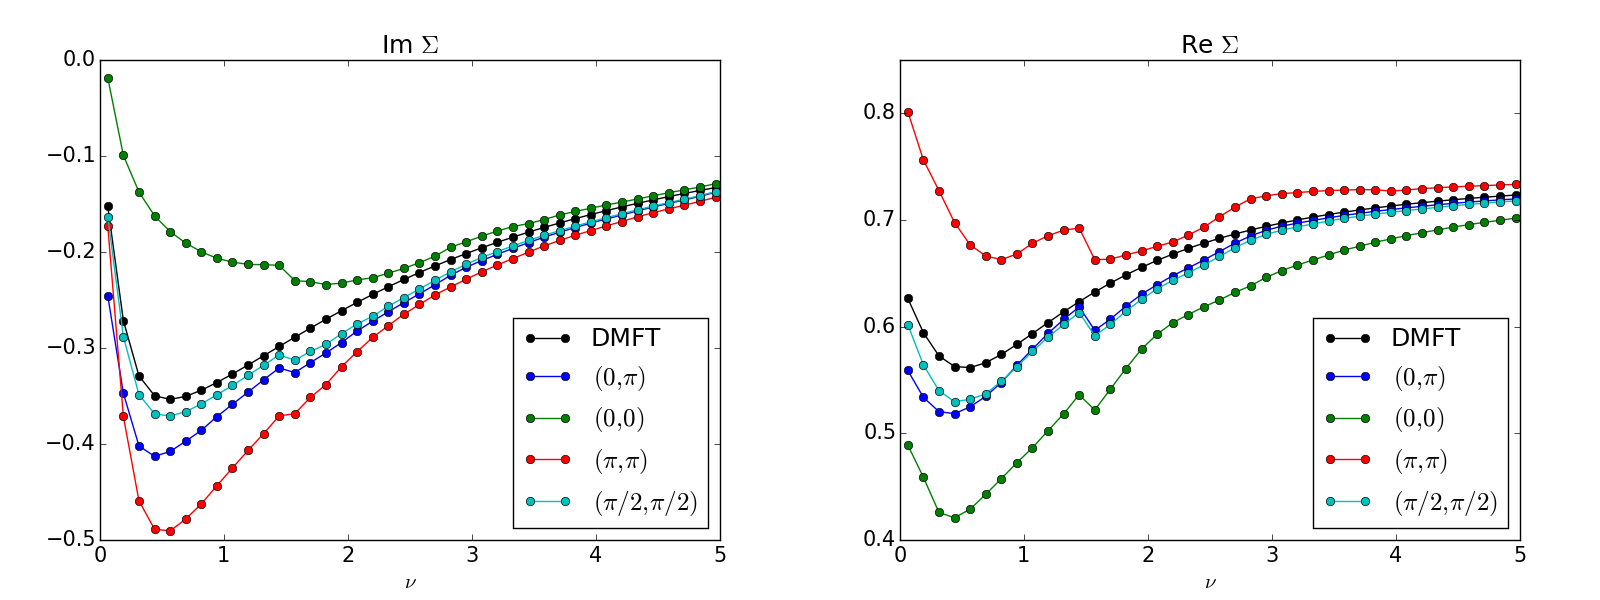
\includegraphics[scale=0.25]{images/Merged_dmf2rg_se_freq.png}
\caption{DMFT and DMF$^2$RG self energy at the critical scale.} \label{dmf2self}
\end{figure}



\subparagraph{Self energy feedback}
\begin{itemize}
\item The self energy suppresses the charge-channel (see Fig. \ref{dmf2rglam}), while being less effective on the AF vertex; 
\item 	The AF channel flow is unusual: it grows towards large coupling value, without "exploding" for a well defined value of critical $\Lambda$. This effect can be possibly due either to the the "interpolative" cutoff used or to a feedback effect of the self energy that avoids a sudden "explosion" of the vertex. 
\item The momentum dependence of the self-energy is relatively modest: there are deviations from the local DMFT self energy, but the self energy remains Fermi-liquid like in all the BZ, see Fig. \ref{dmf2self} Why such a small change of $\Sigma$ has such a large consequence on the flow? 

\item \textbf{TODO}: Study of the effect of the momentum dependence of the self-energy on the bubble. Compare $\nu$ dependent bubble at a given cutoff with and without self energy feedback. Subtract then local bubble to be more consistent. 
\item \textbf{TODO}: How is the ferromagnetism affected by the self energy? Is it a general effect that the self energy suppress the bubble more at $0,0$ than at $\pi,\pi$i? 
\end{itemize} 



%\section{DMF$^2$RG with self-energy}	
%\label{sec:dmf2rgself}
  %Insert some text here. 
\begin{equation}
\label{sdmft}
a = a ;  
\end{equation}


\begin{figure}
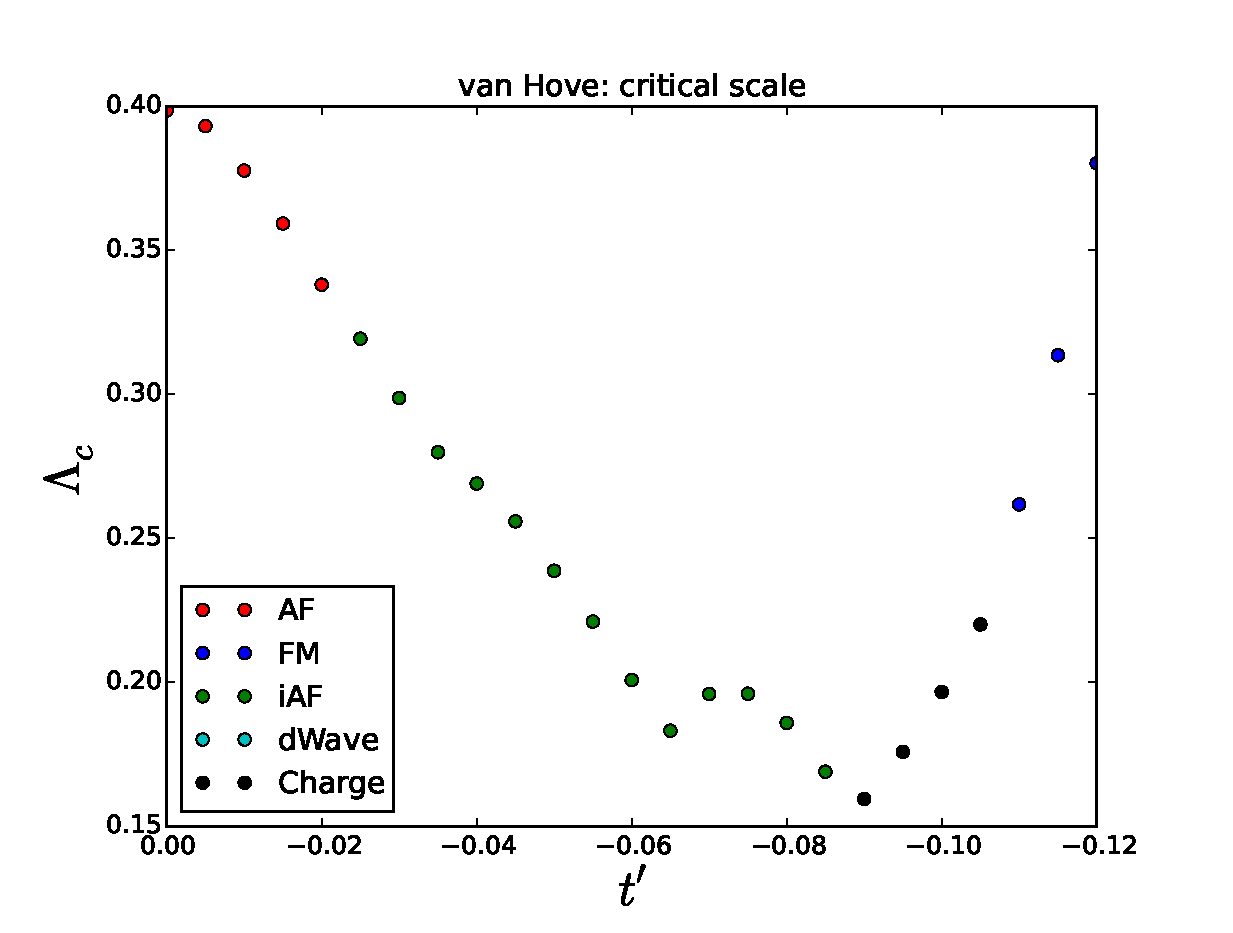
\includegraphics[scale=0.5]{vanHove_scan_critical_lambda_phi.eps}
\caption{Diagrammatic elements used in the text. The Yukawa coupling already refers to the case of spin boson. For a density boson there is a plus sign. } \label{dictionary}

\end{figure}


%\section{Perpendicular ladders}				
%\label{sec:perpendciular}
  %\begin{itemize}

\item Magnetic RPA local effective interaction:
\begin{equation}
  U_{eff}(\Omega) =\int_{\boldsymbol{Q}} \frac{U}{ 1 - U \Pi^{\Omega}_{\boldsymbol{Q}} }
\end{equation}

\item RPA for charge channel:
\begin{equation}
  \Phi_{charge}^{\Omega,\nu,\nu'}(\boldsymbol{Q}) = U_{eff}(\Omega) 
  \left[ 1+  \Pi^{\Omega,\nu}_{\boldsymbol{Q}} U_{eff}(\nu'-\nu) \right]_{\nu,\nu'}^{-1}
\end{equation}

\end{itemize}

\begin{figure}
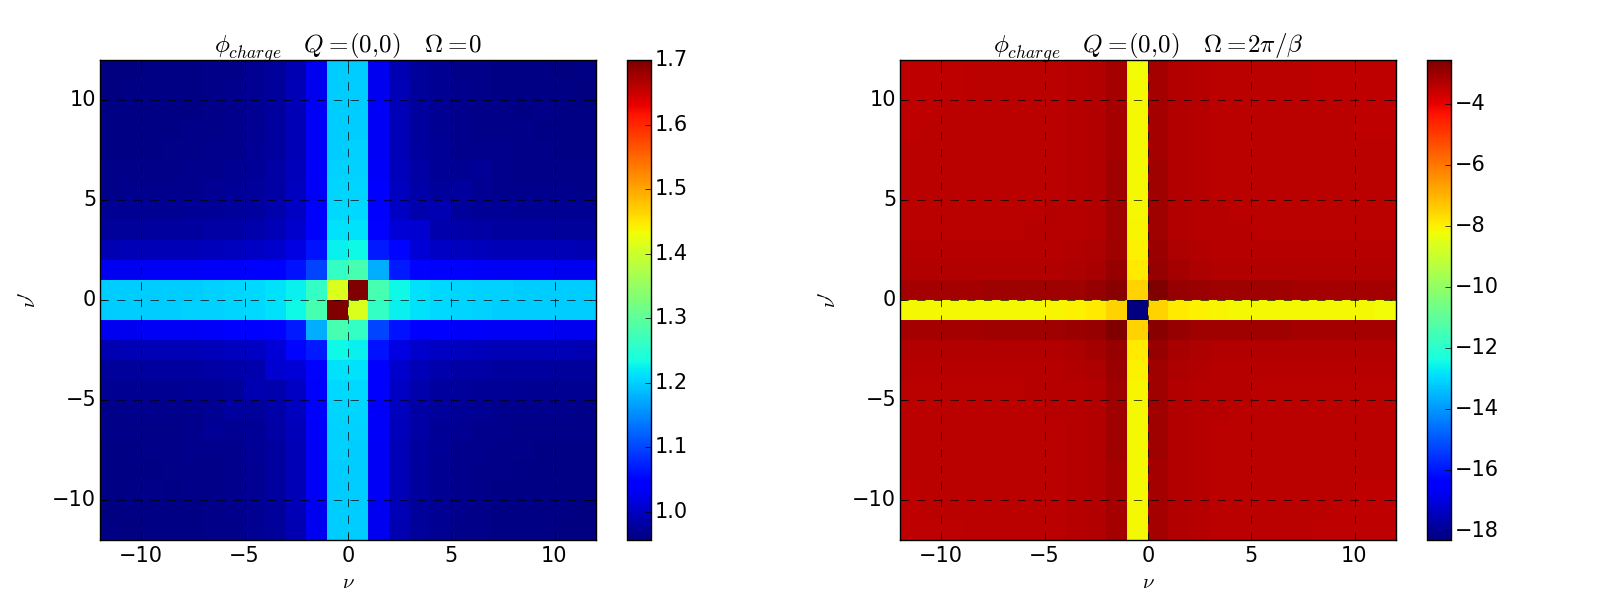
\includegraphics[scale=0.25]{images/Perp_ladder_density.png}
\caption{Charge channel calculated with RPA method for $\Omega=0$ (left) and $\Omega=2\pi/\beta$ (right). }
 \label{Perpladder}
\end{figure}

\begin{figure}
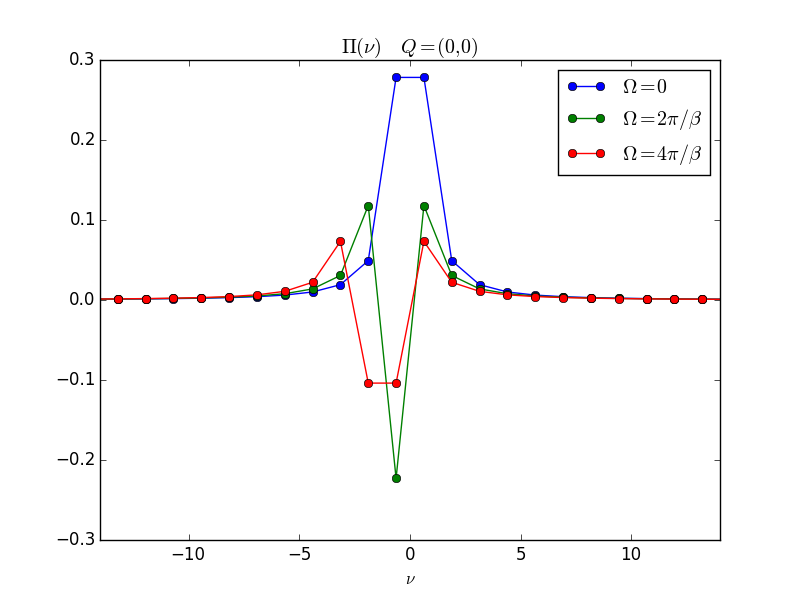
\includegraphics[scale=0.7]{images/Bubble_ph.png}
\caption{PH Bubble as a function of fermionic frequency $\nu$ at $\boldsymbol{Q}=(0,0)$. }
 \label{Perpladder}
\end{figure}

%\section{Self-energy in fRG}				
%\label{sec:frgself}
  %Insert some text here. 
\begin{equation}
\label{sdmft}
a = a ;  
\end{equation}


\begin{figure}
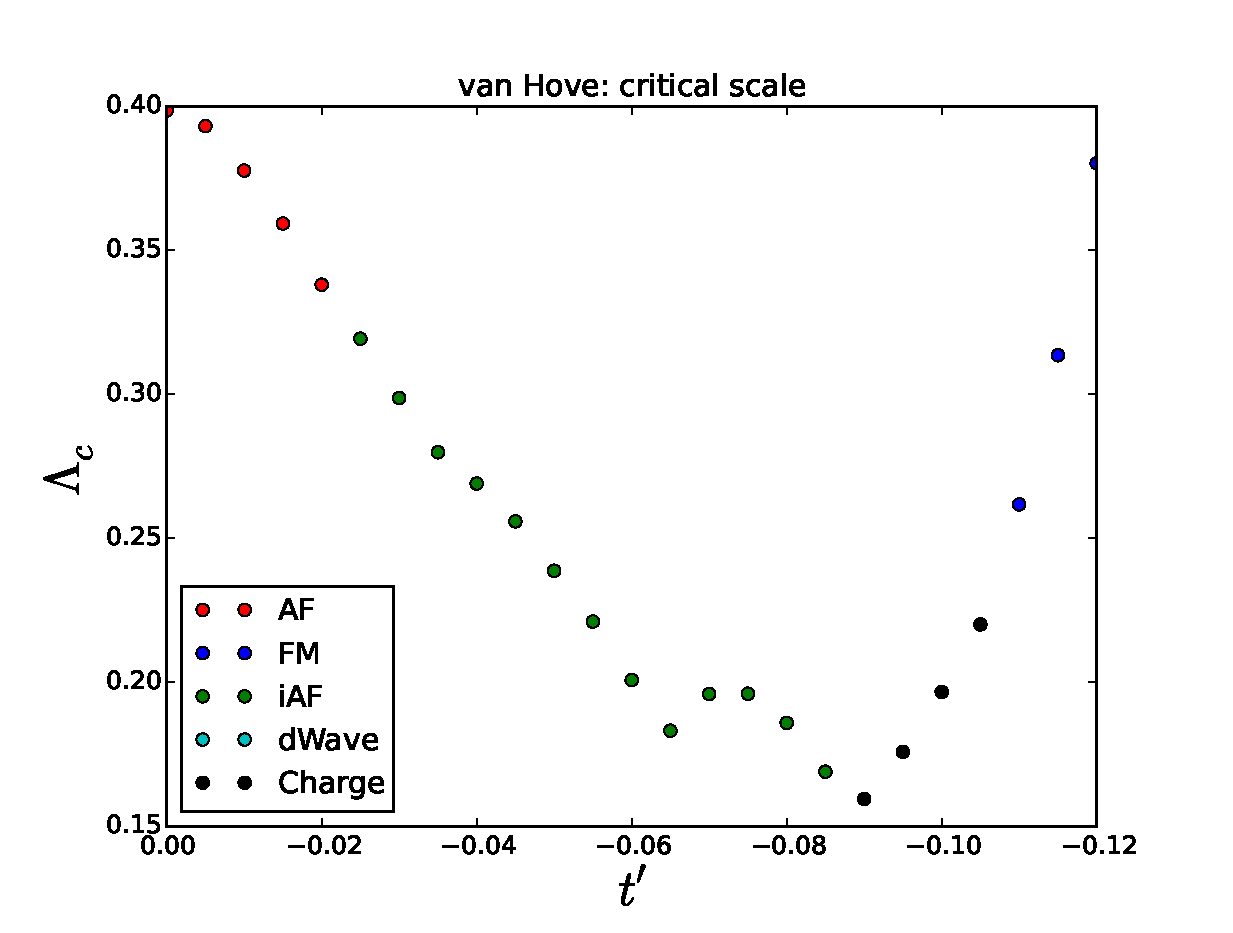
\includegraphics[scale=0.5]{vanHove_scan_critical_lambda_phi.eps}
\caption{Diagrammatic elements used in the text. The Yukawa coupling already refers to the case of spin boson. For a density boson there is a plus sign. } \label{dictionary}

\end{figure}


  \bibliography{refs}

\end{document}
